\documentclass[11pt,a4paper]{article}
\usepackage[utf8]{inputenc}
\usepackage[T1]{fontenc}
\usepackage{lmodern}
\usepackage[a4paper,margin=2.4cm]{geometry}
\usepackage{tikz}
\usetikzlibrary{arrows.meta,positioning,shapes.geometric,fit,calc,backgrounds}
\usepackage{booktabs,xcolor,enumitem,float}
\usepackage[colorlinks=true,linkcolor=blue!50!black,urlcolor=blue!50!black]{hyperref}
\setlength{\parskip}{0.5em}\setlength{\parindent}{0pt}

\definecolor{db}{HTML}{DCE9F7}\definecolor{ui}{HTML}{E6F2E1}\definecolor{ai}{HTML}{FBE8D3}\definecolor{ok}{HTML}{E9E4F5}
\tikzset{
  box/.style={draw,rounded corners=3pt,align=center,minimum height=8mm,inner sep=4pt,font=\small},
  db/.style={box,fill=db},ui/.style={box,fill=ui},ai/.style={box,fill=ai},ck/.style={box,fill=ok},
  arr/.style={-{Latex[length=2mm]},thick},
  note/.style={font=\scriptsize\itshape,align=center}
}
\newcommand{\sql}[1]{\texttt{\small #1}}

\title{Guide du site : explorer Wikipédia (finnois, suédois, anglais)\\avec MariaDB et la recherche vectorielle}
\author{Projet Junction 2026 -- MariaDB $\times$ Wikipedia}
\date{14 novembre 2026}

\begin{document}
\maketitle
\tableofcontents

\section{À quoi sert le site}
Le site est une démonstration construite sur \textbf{MariaDB 11.8} (recherche vectorielle native) et un modèle de langage (Gemini). Il contient des articles Wikipédia sur l'histoire de la Finlande, en trois langues, et propose des outils pour \emph{poser des questions}, \emph{comparer les langues}, \emph{suivre l'évolution des opinions} et \emph{aider les éditeurs}.

\begin{table}[H]\centering\small
\begin{tabular}{@{}lll@{}}\toprule
Page & Pour qui & Ce qu'elle fait\\\midrule
\texttt{/ask} & lecteur & répond à une question avec citations des articles\\
\texttt{/mirror} & lecteur, éditeur & carte des écarts entre langues d'un même sujet\\
\texttt{/stats} & tous & nombre d'articles par langue, sujets en deux ou trois langues\\
\texttt{/neighbors} & lecteur & les 10 articles les plus proches d'un article, dans toutes les langues\\
\texttt{/drift} & lecteur & comment l'opinion d'un article a changé dans le temps\\
\texttt{/gaps} & éditeur & sections présentes dans une langue, absentes d'une autre\\
\texttt{/refs} & éditeur & référence déjà utilisée ailleurs pour un paragraphe non sourcé\\
\texttt{/links} & éditeur & liens internes manquants, articles orphelins\\
\texttt{/consistency} & éditeur & passages d'articles différents qui se contredisent peut-être\\\bottomrule
\end{tabular}
\end{table}

Tout est affiché de façon transparente : chaque page d'outil montre la requête SQL utilisée. Le site ne dit jamais « qui a raison » : il fournit des pistes que l'éditeur ou le lecteur vérifie.

\section{Vue d'ensemble technique}
\begin{figure}[H]\centering
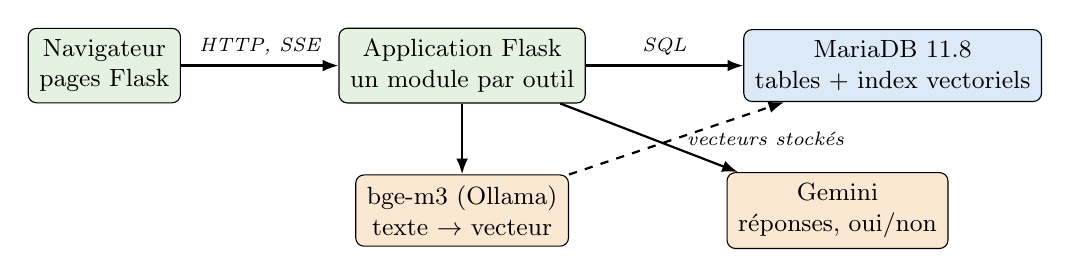
\begin{tikzpicture}[node distance=9mm and 20mm]
\node[ui](nav){Navigateur\\pages Flask};
\node[ui,right=of nav](flask){Application Flask\\un module par outil};
\node[db,right=of flask](maria){MariaDB 11.8\\tables + index vectoriels};
\node[ai,below=of flask](emb){bge-m3 (Ollama)\\texte $\to$ vecteur};
\node[ai,right=of emb](gem){Gemini\\réponses, oui/non};
\draw[arr](nav)--node[above,note]{HTTP, SSE}(flask);
\draw[arr](flask)--node[above,note]{SQL}(maria);
\draw[arr](flask)--(emb);\draw[arr](flask)--(gem);
\draw[arr,dashed](emb)--node[right,note]{vecteurs stockés}(maria);
\end{tikzpicture}
\caption{Architecture. Le navigateur reçoit les résultats au fil de l'eau (SSE).}
\end{figure}

\subsection{Les données}
\begin{itemize}[nosep]
\item \textbf{29\,460 articles} : 19\,285 finnois, 4\,921 suédois, 5\,254 anglais ; 18\,875 sujets, dont 2\,919 existent dans les trois langues (même identifiant Wikidata).
\item \textbf{Un vecteur par article} (\texttt{article\_vector}) et \textbf{un par section} (\texttt{chunk\_vector}, 91\,686 sections) ; pour le finnois, \textbf{un par paragraphe} (\texttt{para\_vector}, 132\,446), avec ses références (191\,421) et ses liens sortants (550\,412).
\item Un \textbf{historique de versions} des articles pour la page \texttt{/drift}.
\end{itemize}

\begin{figure}[H]\centering
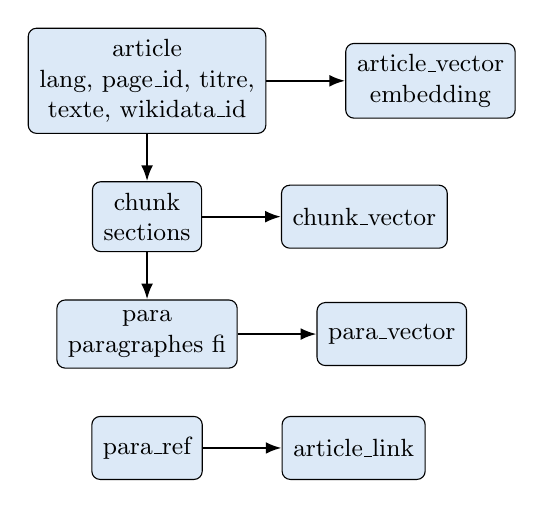
\begin{tikzpicture}[node distance=6mm and 10mm]
\node[db](a){article\\lang, page\_id, titre,\\texte, wikidata\_id};
\node[db,right=of a](av){article\_vector\\embedding};
\node[db,below=of a](c){chunk\\sections};
\node[db,right=of c](cv){chunk\_vector};
\node[db,below=of c](p){para\\paragraphes fi};
\node[db,right=of p](pv){para\_vector};
\node[db,below=of p](pr){para\_ref};
\node[db,right=of pr](al){article\_link};
\draw[arr](a)--(av);\draw[arr](a)--(c);\draw[arr](c)--(cv);\draw[arr](c)--(p);
\draw[arr](p)--(pv);\draw[arr](pr)--(al);
\end{tikzpicture}
\caption{Tables principales (le trait part d'un article vers ce qui le découpe).}
\end{figure}

\subsection{La recherche vectorielle en une image}
Un texte est transformé par \emph{bge-m3} en un vecteur de nombres ; deux textes de sens proche (même dans deux langues) ont des vecteurs proches. La proximité est la \textbf{distance cosinus} : 0 = identique, plus la valeur est grande, plus les sens diffèrent. MariaDB trouve les voisins les plus proches grâce à un index HNSW.

\begin{figure}[H]\centering
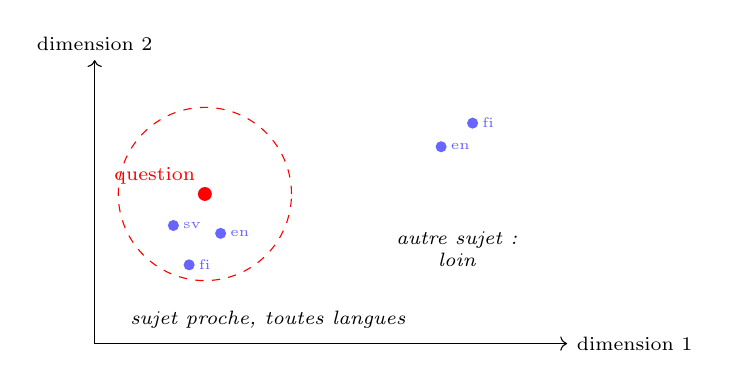
\begin{tikzpicture}
\draw[->](0,0)--(6,0)node[right,font=\scriptsize]{dimension 1};\draw[->](0,0)--(0,3.6)node[above,font=\scriptsize]{dimension 2};
\foreach \x/\y/\l in {1.2/1.0/fi,1.6/1.4/en,1.0/1.5/sv,4.8/2.8/fi,4.4/2.5/en}{\fill[blue!60](\x,\y)circle(2pt)node[right,font=\tiny]{\l};}
\fill[red](1.4,1.9)circle(2.5pt)node[above left,font=\scriptsize]{question};
\draw[red,dashed](1.4,1.9)circle(1.1);
\node[note]at(4.6,1.2){autre sujet :\\loin};
\node[note]at(2.2,0.3){sujet proche, toutes langues};
\end{tikzpicture}
\caption{La question tombe près des textes de même sens, quelle que soit leur langue.}
\end{figure}

La forme de requête utilisée partout : la recherche d'abord dans une sous-requête, la jointure ensuite.
\begin{center}\sql{SELECT ... FROM (SELECT ..., VEC\_DISTANCE\_COSINE(embedding, ?) AS d FROM article\_vector ORDER BY d LIMIT n) v JOIN article ...}\end{center}
\textbf{Limite connue :} le cache du graphe HNSW (\texttt{mhnsw\_max\_cache\_size}, 16~Mo) est plus petit que l'index, donc deux connexions peuvent lire des graphes légèrement différents (rappel mesuré : 0,94 à 0,96 en moyenne). Un cache plus grand est le remède, non appliqué.

\section{Pour le lecteur}
\subsection{\texttt{/ask} : poser une question}
\begin{figure}[H]\centering
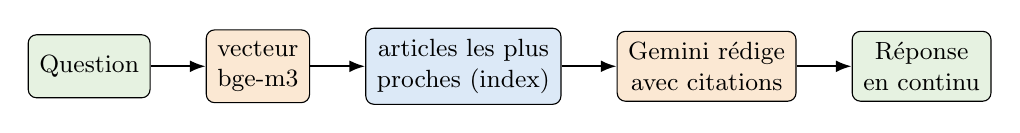
\begin{tikzpicture}[node distance=7mm]
\node[ui](q){Question};
\node[ai,right=of q](e){vecteur\\bge-m3};
\node[db,right=of e](s){articles les plus\\proches (index)};
\node[ai,right=of s](g){Gemini rédige\\avec citations};
\node[ui,right=of g](r){Réponse\\en continu};
\foreach \a/\b in {q/e,e/s,s/g,g/r}\draw[arr](\a)--(\b);
\end{tikzpicture}
\caption{Principe RAG : retrouver d'abord, rédiger ensuite à partir des articles trouvés seulement.}
\end{figure}
On peut restreindre à une langue. Les sources, leurs distances, les temps (embedding, recherche, génération) et le SQL sont affichés.

\subsection{\texttt{/mirror} : le miroir des langues}
Pour chaque sujet existant en deux langues, une requête SQL calcule la distance entre les deux vecteurs d'article. Les sujets sont placés sur une carte 2D (projection PCA calculée une fois) ; plus l'écart est grand, plus les deux langues racontent un sujet différemment.

\begin{figure}[H]\centering
\begin{tikzpicture}[node distance=7mm]
\node[db](p){paires d'articles\\même wikidata\_id};
\node[db,right=of p](d){distance cosinus\\des 2 vecteurs};
\node[ui,right=of d](m){carte + liste\\triée par écart};
\node[ai,below=of m](n){note de Gemini :\\« seulement en A / en B »};
\draw[arr](p)--(d);\draw[arr](d)--(m);\draw[arr](m)--node[right,note]{clic sur une paire}(n);
\end{tikzpicture}
\caption{La note de comparaison cite des extraits des deux textes ; rien n'est traduit.}
\end{figure}

\subsection{\texttt{/stats} et \texttt{/neighbors}}
\texttt{/stats} compte les articles par langue et les sujets présents en deux ou trois langues. \texttt{/neighbors} prend un article et affiche ses 10 plus proches par le sens (index vectoriel), toutes langues confondues ; un clic saute à l'un d'eux.

\subsection{\texttt{/drift} : la dérive d'opinion}
Sous le capot, un module \texttt{decisions.py} (sans page propre) interroge une API de décision de Gemini qui renvoie la probabilité qu'un texte soutienne une affirmation ; un texte vide donne $[0,0,1,0,0]$ sans appel.

On pose une question ; le site retrouve les articles pertinents, relit \textbf{toutes leurs versions successives}, mesure la position de chaque version sur des affirmations extraites, et repère les \textbf{points de changement}.

\begin{figure}[H]\centering
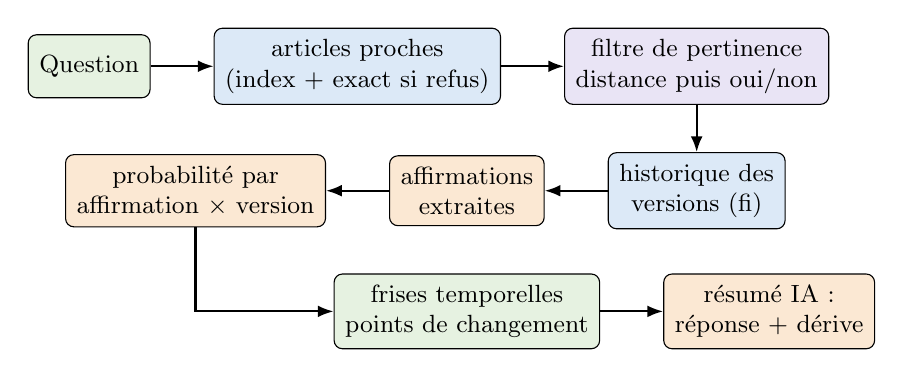
\begin{tikzpicture}[node distance=6mm and 8mm]
\node[ui](q){Question};
\node[db,right=of q](r){articles proches\\(index + exact si refus)};
\node[ck,right=of r](f){filtre de pertinence\\distance puis oui/non};
\node[db,below=of f](h){historique des\\versions (fi)};
\node[ai,left=of h](c){affirmations\\extraites};
\node[ai,left=of c](p){probabilité par\\affirmation $\times$ version};
\node[ui,below=of c](t){frises temporelles\\points de changement};
\node[ai,right=of t](s){résumé IA :\\réponse + dérive};
\draw[arr](q)--(r);\draw[arr](r)--(f);\draw[arr](f)--(h);\draw[arr](h)--(c);\draw[arr](c)--(p);
\draw[arr](p)|-(t);\draw[arr](t)--(s);
\end{tikzpicture}
\caption{Chaîne complète. Les étapes arrivent en direct dans la page.}
\end{figure}

\paragraph{Filtre de pertinence en deux temps.}
(1) refus si le meilleur article est à plus de 0,48 de la question ; les articles à plus de 0,07 du meilleur sont écartés ; (2) une question oui/non par candidat (« cet article traite-t-il du sujet demandé ? », seuil 0,5). Sur 7 questions : sujet hors champ (coupe du monde 1998) et question mêlée (Napoléon, traité de 1763) refusées ; questions pertinentes gardent 1 à 5 articles.

\paragraph{Lire la page.} Une ligne par affirmation, avec la frise de ses versions ; les points colorés sont des changements (clic pour la preuve), les titres de changement sont triés par date ; export JSON et lien copiable ; rejeu instantané : \texttt{?fixture=1\&fast=1}.

\section{Pour l'éditeur (outils de niveau B)}
Les quatre outils partagent la même idée : un voisinage vectoriel propose des pistes, une question oui/non (mise en cache) ou un seuil les trie, et l'éditeur décide.

\subsection{\texttt{/gaps} : sections manquantes entre langues}
\begin{figure}[H]\centering
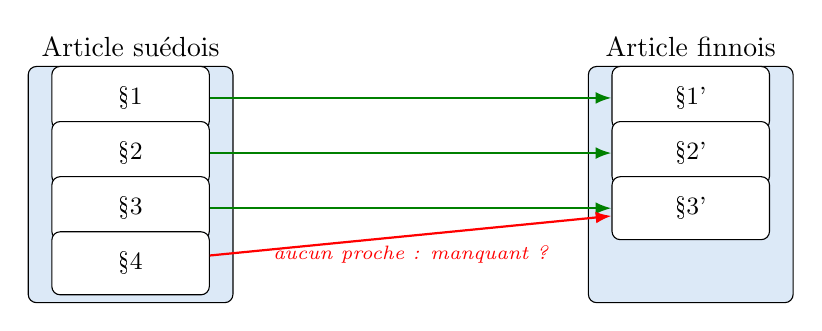
\begin{tikzpicture}
\node[db,minimum width=2.6cm,minimum height=3cm,label=above:Article suédois](sv){};
\node[db,minimum width=2.6cm,minimum height=3cm,right=4.5cm of sv,label=above:Article finnois](fi){};
\foreach \i/\y in {1/1.1,2/0.4,3/-0.3,4/-1.0}{\node[box,fill=white,minimum width=2cm](s\i)at($(sv)+(0,\y)$){§\i};}
\foreach \i/\y in {1/1.1,2/0.4,3/-0.3}{\node[box,fill=white,minimum width=2cm](f\i)at($(fi)+(0,\y)$){§\i'};}
\draw[arr,green!50!black](s1)--(f1);\draw[arr,green!50!black](s2)--(f2);\draw[arr,green!50!black](s3)--(f3);
\draw[arr,red](s4)--node[below,note]{aucun proche : manquant ?}(f3);
\end{tikzpicture}
\caption{Chaque section est reliée à sa plus proche dans l'autre article ; une grande distance signale un manque.}
\end{figure}
Sans modèle de langage, par un calcul de distance exact entre les sections des deux articles. \textbf{Deux niveaux} : au-dessus de 0,40 « probablement manquante » (6 sur 7 vraiment manquantes sur 64 sections étiquetées), entre 0,32 et 0,40 « à regarder » (environ une sur trois). Les listes de références sont écartées.

\subsection{\texttt{/refs} : emprunter une référence}
\begin{figure}[H]\centering
\begin{tikzpicture}[node distance=7mm]
\node[ui](p){paragraphe\\sans référence};
\node[db,right=of p](k){5 paragraphes proches\\avec référence\\(autres articles)};
\node[ck,right=of k](y){« même fait ? »\\oui/non};
\node[ui,right=of y](o){référence proposée\\(« non confirmée » sinon)};
\foreach \a/\b in {p/k,k/y,y/o}\draw[arr](\a)--(\b);
\end{tikzpicture}
\caption{Wikipédia ne peut pas se citer elle-même : on emprunte la source qu'un autre article utilise.}
\end{figure}
C'est une piste, pas une citation : l'éditeur ouvre la source. Test sur 50 paragraphes dont la référence a été masquée : 13 avaient la même référence ailleurs ; retrouvée par la recherche dans 11 cas, confirmée par le contrôle dans 3.

\subsection{\texttt{/links} : liens internes}
Deux vues. \textbf{Proches mais non liés} : les articles proches par le sens sans lien dans aucun sens, avec le paragraphe où le lien irait. \textbf{Moins de liens entrants} : les articles orphelins, avec cinq endroits d'où y faire un lien.

\begin{figure}[H]\centering
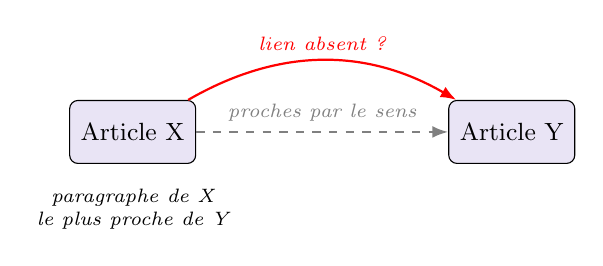
\begin{tikzpicture}[node distance=12mm]
\node[ck](x){Article X};\node[ck,right=3.2cm of x](y){Article Y};
\draw[arr,gray,dashed](x)--node[above,note]{proches par le sens}(y);
\draw[arr,red](x)to[bend left=30]node[above,note]{lien absent ?}(y);
\node[note,below=2mm of x]{paragraphe de X\\le plus proche de Y};
\end{tikzpicture}
\caption{Les voisins déjà liés (dans un sens ou l'autre) sont retirés avant l'affichage.}
\end{figure}
Test : 100 liens masqués puis retrouvés en top-10 : 29\,\% sur un sous-ensemble de 917 articles, 8\,\% sur les 19\,285 articles.

\subsection{\texttt{/consistency} : contradictions possibles}
\begin{figure}[H]\centering
\begin{tikzpicture}[node distance=6mm]
\node[ui](s){section\\d'un article};
\node[db,right=of s](n){sections proches\\d'autres articles};
\node[ck,right=of n](q1){même sujet\\précis ?};
\node[ck,right=of q1](q2){valeurs\\incompatibles ?};
\node[ui,right=of q2](r){deux passages\\côte à côte};
\foreach \a/\b in {s/n,n/q1,q1/q2,q2/r}\draw[arr](\a)--(\b);
\node[note,below=2mm of q2]{score = P(même sujet)$\times$P(incompatible)\\$\geq 0{,}5$ « peuvent différer » ; $0{,}3$--$0{,}5$ « à regarder »};
\end{tikzpicture}
\caption{Chaque passage est précédé du titre de l'article et de la section, ce qui évite de confondre deux homonymes.}
\end{figure}
L'outil affiche peu de paires et ne dit jamais laquelle est juste. Sur 800 paires : une signalée à $\geq 0{,}5$, et c'était une vraie divergence (fusion de Tele Finland en 2005 ou 2017).

\section{Comment lire les nombres}
\begin{itemize}[nosep]
\item \textbf{Distance} : 0 identique ; vers 0,4--0,5 déjà « un peu loin » ; au-delà de 0,5 en général sans rapport.
\item \textbf{Probabilité} (oui/non) : entre 0 et 1, seuil de décision 0,5 sauf mention.
\item \textbf{Précision} annoncée pour les outils B : établie sur de petits échantillons étiquetés par le modèle qui a écrit les outils, non par des éditeurs de Wikipédia.
\end{itemize}

\section{Limites}
\begin{itemize}[nosep]
\item Rappel de l'index vectoriel imparfait (cache trop petit), voir plus haut.
\item Opinion drift : historique disponible pour peu d'articles ; filtre de pertinence grossier.
\item B2 et B3 : résultats modestes, présentés comme des pistes ; B4 : très peu de volume.
\item Aucune vérification de rendu dans un navigateur réel n'a pu être faite pour ces pages (extension Chrome non connectée) ; les API et le JavaScript ont été testés par script.
\end{itemize}

\section{Lancer le site}
Copier \texttt{.env.example} en \texttt{.env} et y mettre \texttt{GOOGLE\_API\_KEY} ; exécuter \texttt{scripts/setup.sh} une fois, puis \texttt{scripts/run.sh}. Détails : \texttt{docs/running.md}. Vérifications des outils B : \texttt{scripts/eval\_tier\_b.py} et \texttt{docs/tier-b-checks.md}.
\end{document}
